\documentclass{beamer}
% \usetheme{madrid}

% Packages
%%%%%%%%%%%%%%%%%%%%%%%%%%%%%%%%%%%%%%%%%%%%%%%%%%%%%%%%%%%%%%%%%%%%%%%%%%%%%%%%
\usepackage{calc}
\usepackage{amsmath, amssymb, amsthm} 
\usepackage{parskip}
\usepackage{color,hyperref}
\usepackage{epsfig}
\usepackage{subfigure}
\usepackage{verbatim}
\usepackage{rotating}
% Add my definitions file
\usepackage{kky}
\usepackage{hastieDefns}
\usepackage{multicol}
\usepackage{ifthen}
\usepackage{bbm}
\usepackage{siunitx}
\newenvironment{packed_enum}{
\begin{enumerate}
\setlength{\itemsep}{1pt}
\setlength{\parskip}{0pt}
\setlength{\parsep}{0pt}
}{\end{enumerate}}
%%%%%%%%%%%%%%%%%%%%%%%%%%%%%%%%%%%%%%%%%%%%%%%%%%%%%%%%%%%%%%%%%%%%%%%%%%%%%%%%
% 
% \newcommand{\simul}{\Phi}
% \newcommand{\simdata}{\mathbf{\tilde{X}}}
% \newcommand{\obsdata}{\bf X_{obs}}
% \newcommand{\likl}{\mathcal{L}}
% \newcommand{\estlikl}{\mathcal{\hat{L}}}
% \newcommand{\vari}{\sigma^2_\rho}
% \newcommand{\QQ}{\mathcal{Q}}
% \DeclareMathOperator*{\argmin}{arg\,min}

\definecolor{darkblue}{rgb}{0.0,0.0,0.7}
\hypersetup{colorlinks,breaklinks,
            linkcolor=darkblue,urlcolor=darkblue,
            anchorcolor=darkblue,citecolor=darkblue}

\usepackage{kky}
\usepackage{hastieDefns}

\setbeamertemplate{sidebar right}{}
\setbeamertemplate{footline}{%
\hfill\usebeamertemplate***{navigation symbols}
\hspace{1cm}\insertframenumber{}/\inserttotalframenumber}

\newcommand{\toworkon}[1]{\textcolor{magenta}{[#1]}}
% \newcommand{\toworkon}[1]{}

%% Begin Content
%% =============


\newcommand{\insertTableRealData}{
\begin{table*}
\centering
\begin{tabular}{l|c|c|c|c|c|c|c|c}
Dataset ($D$, $n$) & \addkrr & \krr & \knn & \nw & \locallin & \localquad & \gp  & \svr \\
\hline \\[-0.16in]
\hline 
Speech ($21$, $520$) & $\bf{0.02269}$ & $0.02777$ & $0.09348$ 
  & $0.11207$ & $0.03373$ 
        & $0.02407$ & $0.02531$ & $0.22431$  \\
\hline
Music ($90$, $1000$) & $\bf{0.91627}$ & $0.91922$ & $1.00001$ 
      & $1.05745$ & $1.25805$ 
        & $1.06482$ & $0.94329$ & $1.07009$ \\
\hline
Tele-motor ($19$, $300$) & $\bf{0.06059}$ & $0.06488$ & 
  $0.13957$ & $0.20119$ 
  & $0.09455$ & $0.08774$ & $0.06678$ & $0.38038$ \\
\hline
Housing ($12$, $256$) & $\bf{0.31285}$ & $0.35947$ & $0.43619$ & $0.42087$ 
  & $\bf{0.31219}$ & $0.35061$ & $0.67566$ & $1.15272$ \\
\hline
Blog ($91$, $700$) & $\bf{1.43288}$ & $1.53227$ & $1.73545$ & $1.49305$ & $1.69234$ 
     & $1.71321$ & $1.64429$ & $1.66705$ \\
\hline
Forest Fires ($10$, $210$) & $0.30675$ & $0.32618$ & $0.40565$ & $0.37199$ 
   & $0.35462$ & $0.33881$ & $\bf{0.29038}$ & $0.70154$ \\
\hline
Propulsion ($15$, $400$) & $0.04167$ & $0.01396$ & $0.15760$ & $0.11237$ & $0.182345$ &
             $0.19212$ & $\bf{0.00355}$ & $0.74511$ \\
\hline
\end{tabular}
\caption{
The test set errors of all methods on 7 datasets from the UCI repository.
The dimensionality and number of training points is indicated with the dataset.
The best method(s) for each dataset are in bold font. \addkrr gives the best
results in most of the datasets and is within the top 3 in all of the datasets.
In the Forest Fires dataset it is only slightly worse than \gp. In the
Propulsion dataset, \gp seems to significantly outperform all other methods.
}
\label{tb:realData}
\end{table*}
}


\newcommand{\insertFigCompToy}{
\begin{figure}
\centering
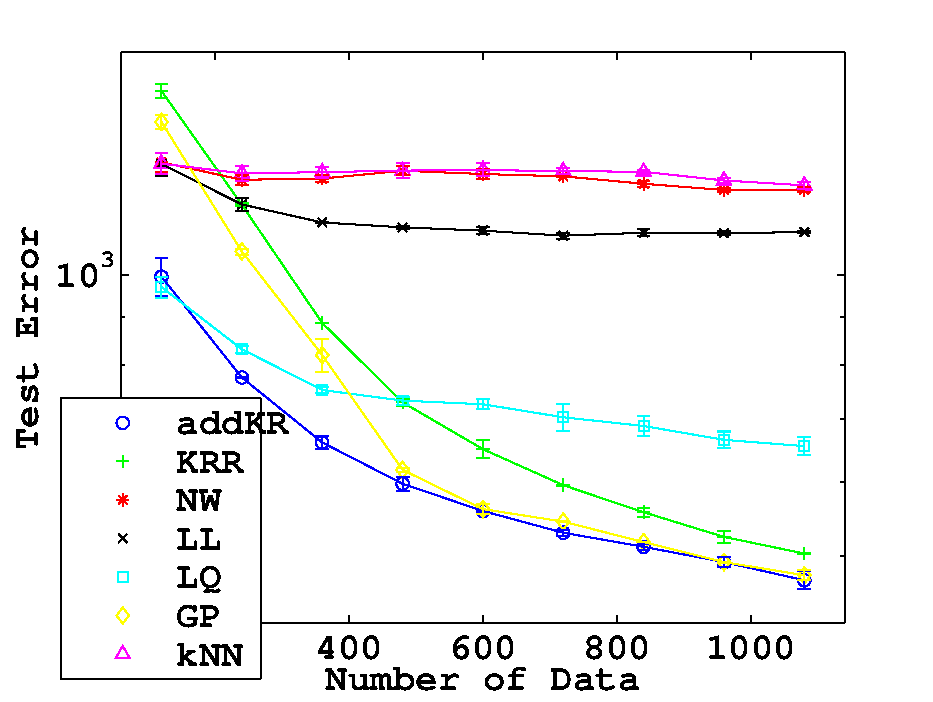
\includegraphics[width=3.2in]{figs/compToy}
\vspace{\imcaptionspace}
\caption[]{\small Comparison of various nonparametric regression methods on a
$20$-dimensional toy dataset. The $x$-axis denotes the number of training data
and the $y$-axis is the test error. }
\vspace{\imtextspace}
\label{fig:compToy}
\end{figure}
}

\newcommand{\insertFigOpt}{
\begin{figure}
\centering
\subfigure[]{
  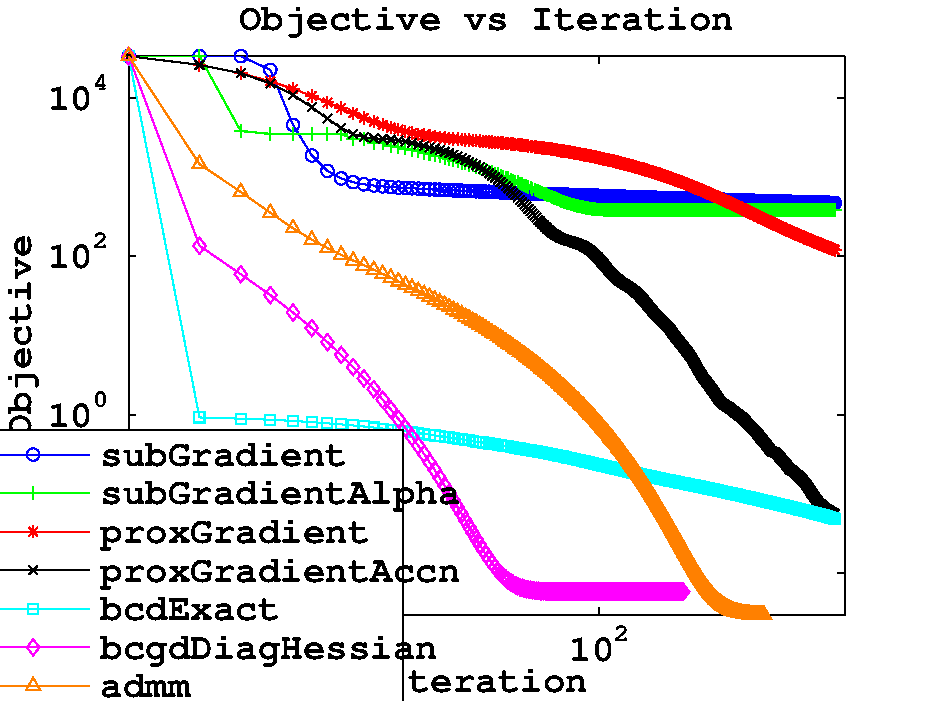
\includegraphics[width=\imarrwtwo]{figs/iteration1000v2} \hspace{\imhsptwo}
  \vspace{\imlabelspace}
  \label{fig:optCompIter}
}
\subfigure[]{
  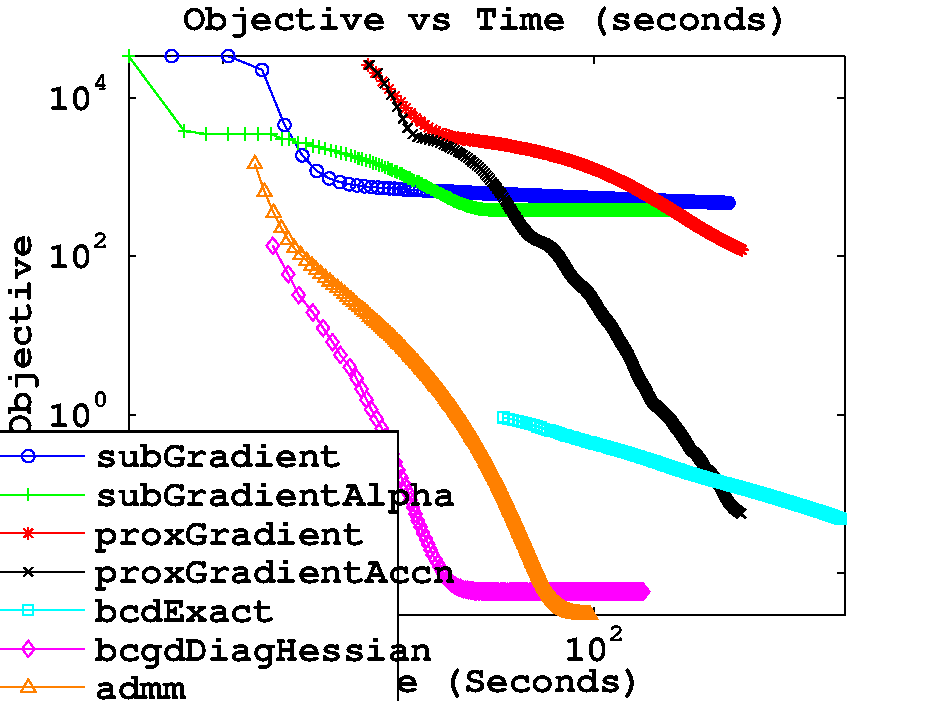
\includegraphics[width=\imarrwtwo]{figs/time1000v2} \hspace{\imhsptwo}
  \vspace{\imlabelspace}
  \label{fig:optCompTime}
}
\caption[]{\small
\subref{fig:optCompIter}: Comparison of the different methods to optimise our
objective. In~\subref{fig:optCompIter} The $x$-axis is the iteration and
in~\subref{fig:optCompTime} the $x$-axis is time. In both figures
 the $y$-axis is the objective. 
Both figures are in log-log scale.
}
\end{figure}
}

\newcommand{\insertFigRegFSel}{
\begin{figure}
\centering
\subfigure[]{
  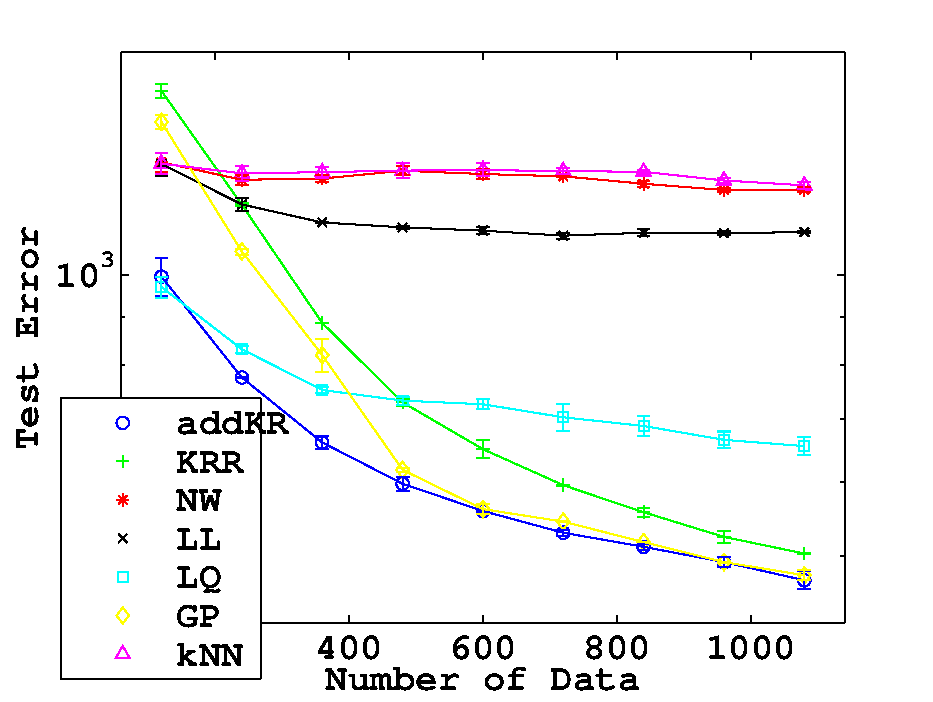
\includegraphics[width=\imarrwtwo]{figs/compToy} \hspace{\imhsptwo}
  \vspace{\imlabelspace}
  \label{fig:compToy}
}
\subfigure[]{
  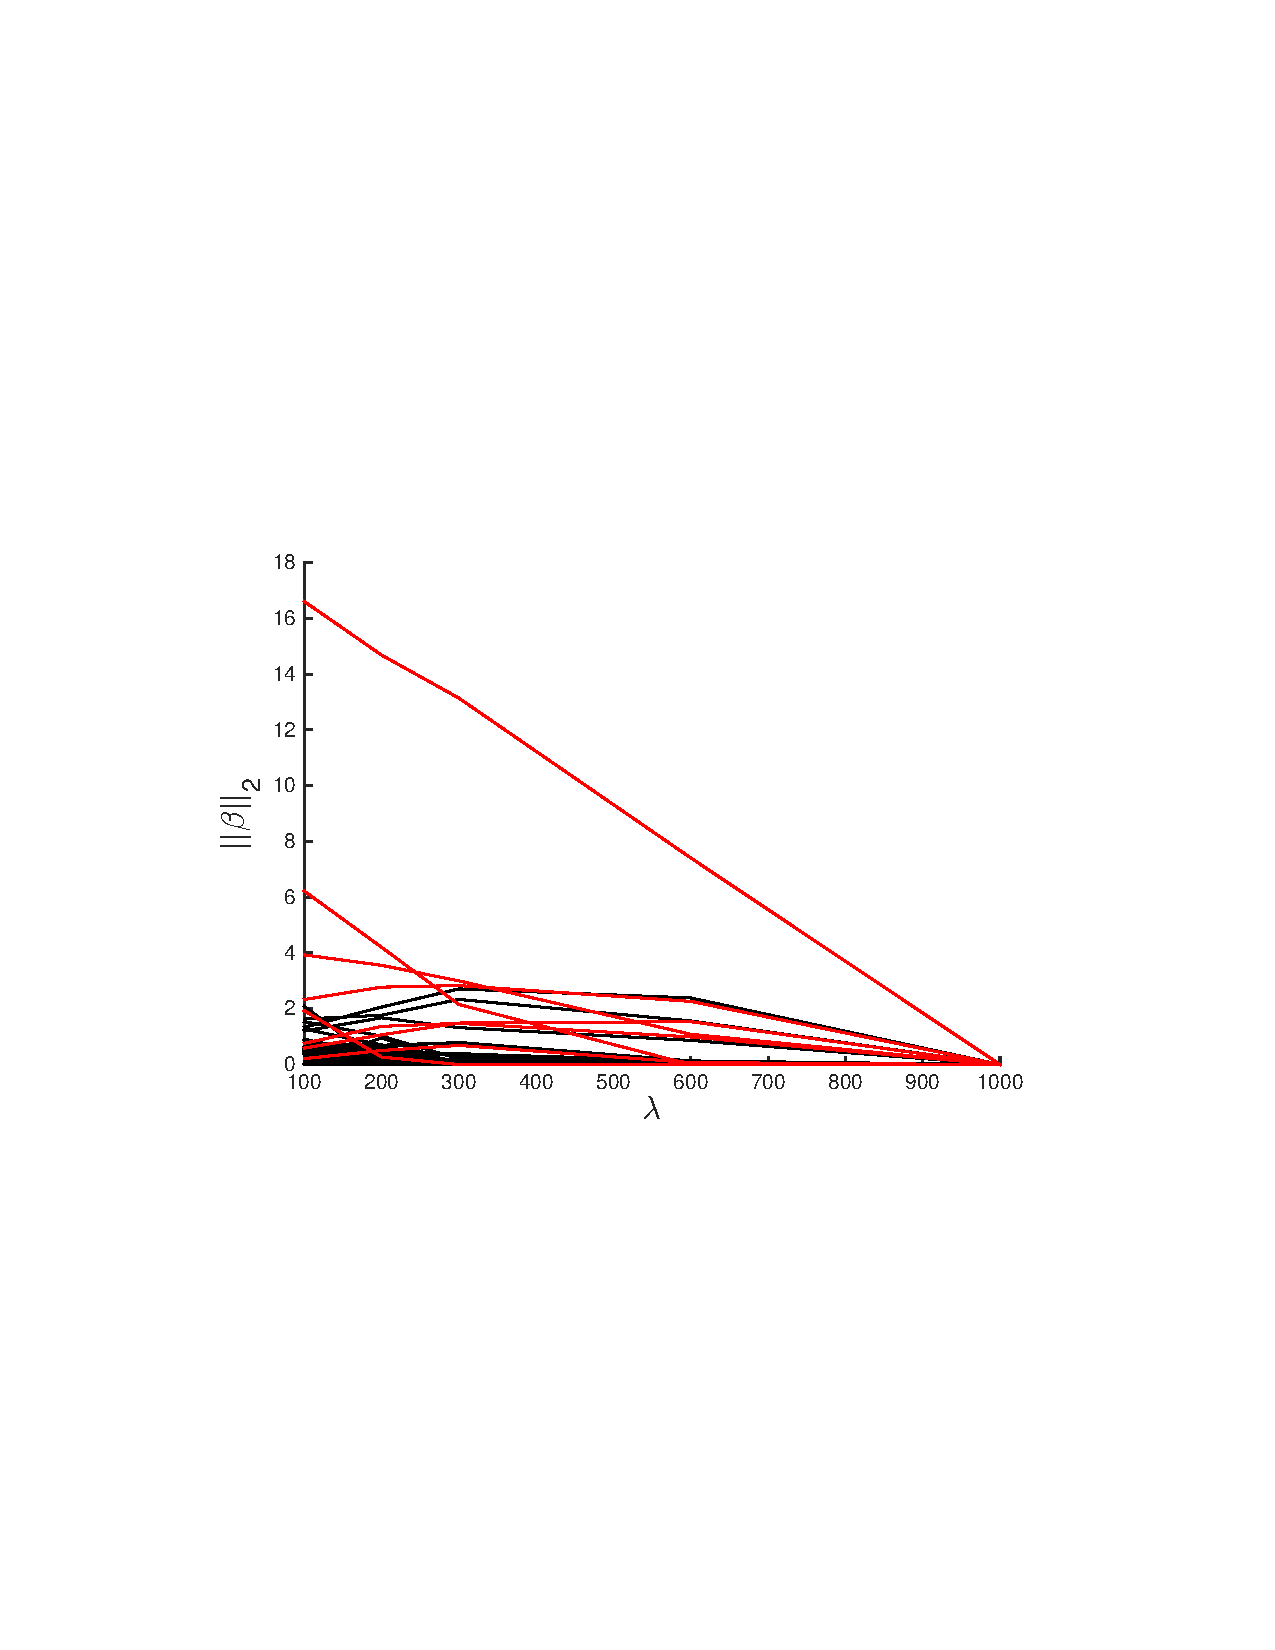
\includegraphics[width=\imarrwtwo]{figs/solnpath600} \hspace{\imhsptwo}
  \vspace{\imlabelspace}
  \label{fig:solnpath}
}
\caption[]{\small
\subref{fig:compToy}: Comparison of \addkrrs using ESP Kernels against other 
nonparametric methods
on a $20$ dimensional toy problem. The $x$-axis denotes the number of training
points and the $y$-axis is the error on a test set.
\subref{fig:solnpath}: Solution path with $n=600$ samples for the synthetic
problem. The $x$-axis shows the regularisation parameter while the $y$-axis
plots $\|\funcj\|_{\Hcalkj} = \|\betaj\|$. The true nonzero functions are
depicted in red. As the figure indicates several of the false functions are
driven to $0$ fast whereas the true functions persist for longer.
}
\end{figure}
}



\newcommand{\insertFigSolnPath}{
\begin{figure}
\centering
% 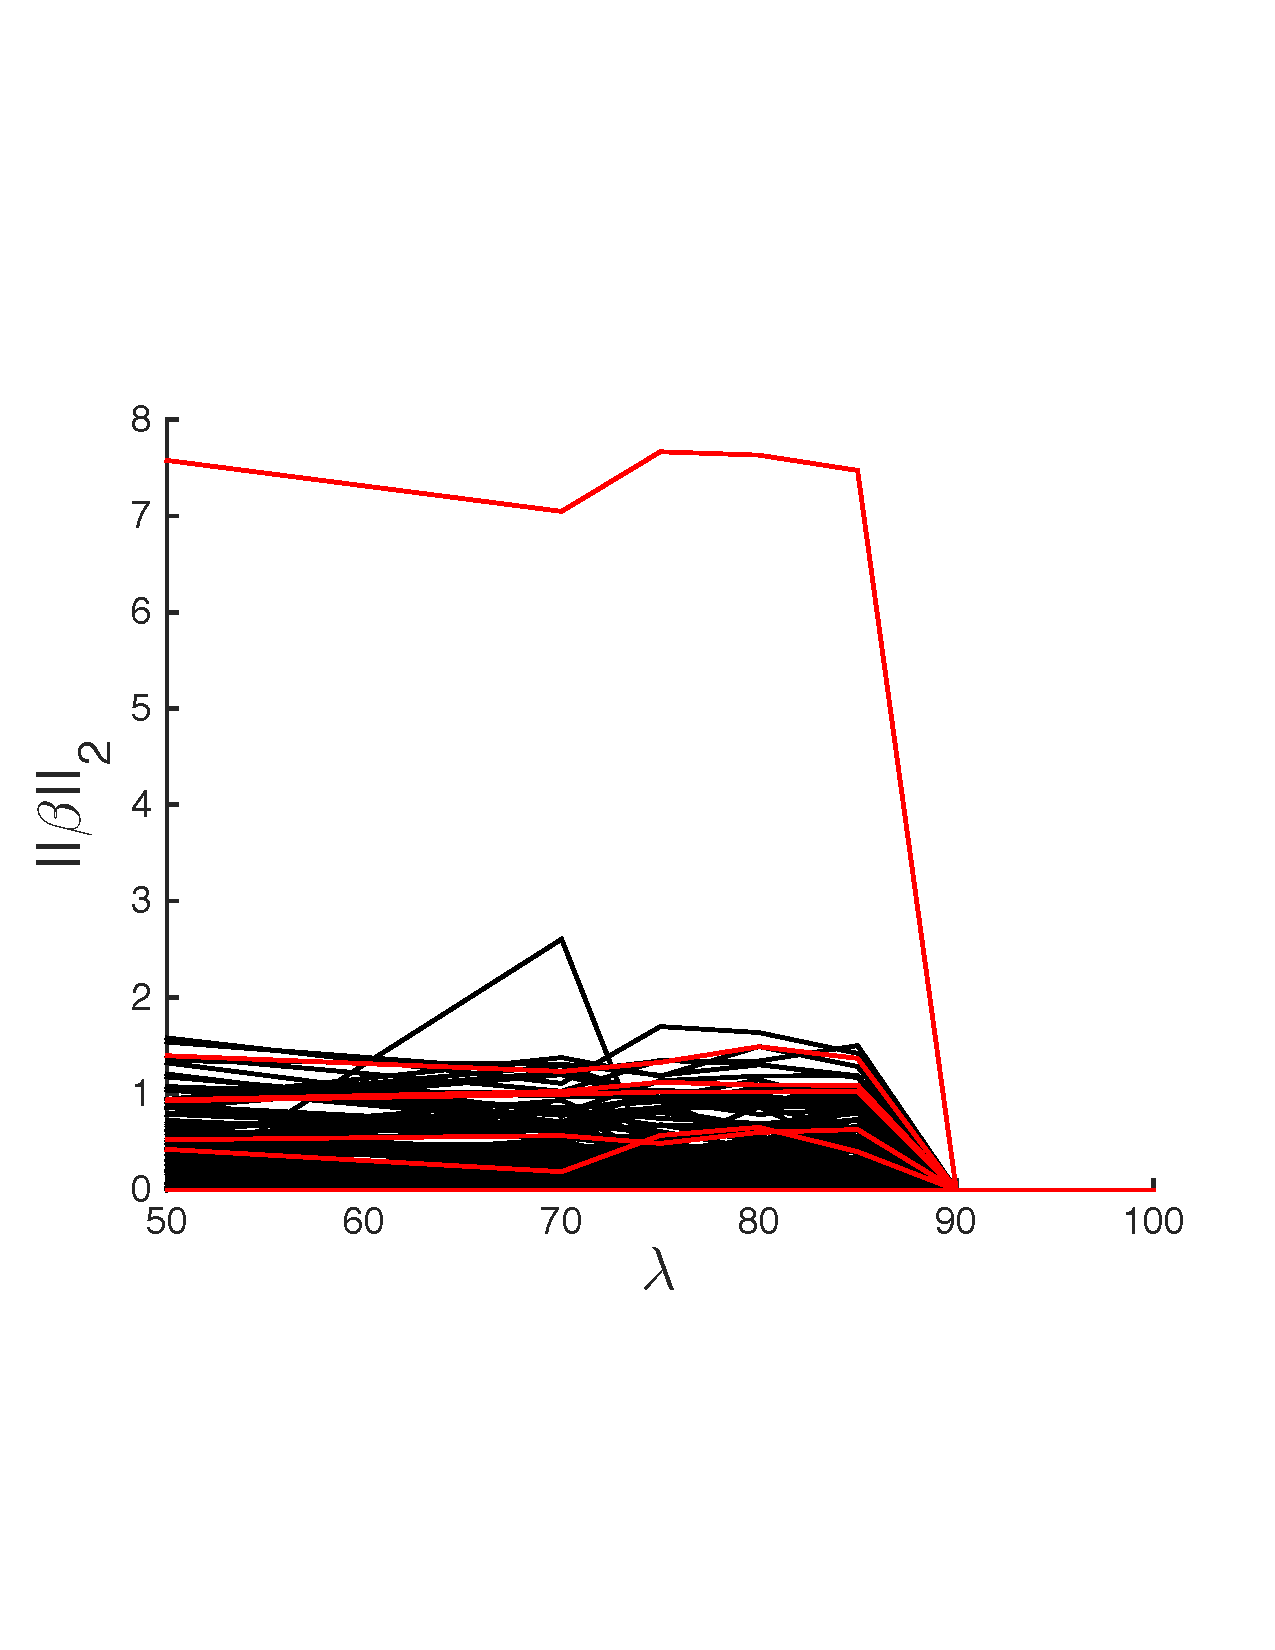
\includegraphics[width=3.4in]{figs/solnpath200.pdf}
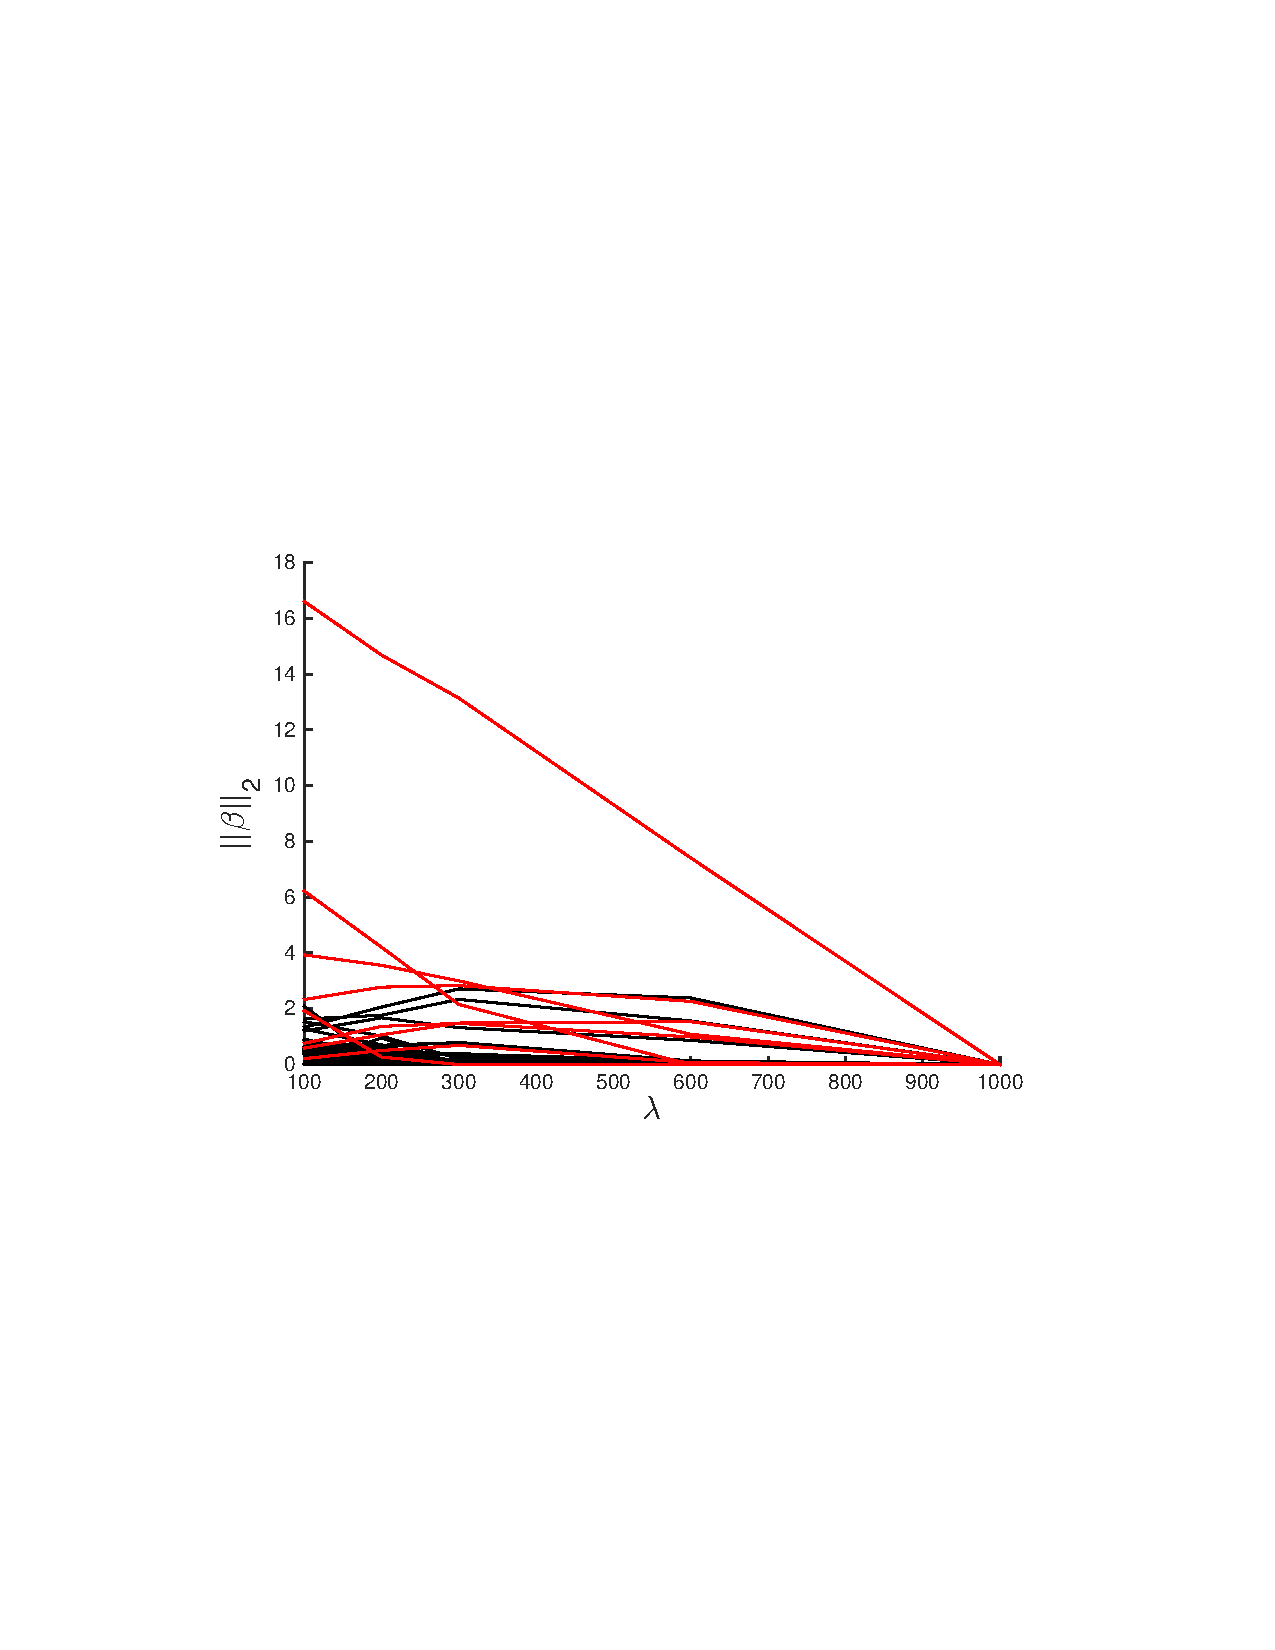
\includegraphics[width=3.2in]{figs/solnpath600.pdf}
\vspace{\imcaptionspace}
\caption[]{\small Solution path with $n=200$ samples (above) and
$n=600$ (below). The $x$-axis shows the regularization parameter,
while the $y$-axis plots $\|\funcj\|_{\Hcalkj} = \|\betaj\|$. 
The true nonzero functiosn are depicted in red. As the figure indicates, several
of the false functions are driven to $0$ fast whereas the true functions
persist for longer.
}
\vspace{\imtextspace}
\label{fig:n200}
\end{figure}
}


\title{Regularised Additive Least Squares Regression}
\author{Calvin \& Kirthevasan}
\date{May 7, 2015}

\begin{document}
\maketitle


\begin{frame}{Nonparametric Regression}

  Given data: $(X_i, Y_i)_{i=1}^n$ \hspace{0.1in} where $(X_i,Y_i)\sim P_{XY}$ \\ 
  Estimate $\func(x) = \EE[Y| X=x]$.
  \vspace{0.1in}
  \pause

  Nonparametric Regression
  \begin{itemize}
    \item Assume only smoothness of $\func$. No parametric form assumed.
    \item E.g.: Nadaraya-Watson, Support Vector Regression, Locally Polynomial
          Regression, Splines etc.
    \vspace{0.15in}
    \pause
    \item \textbf{Kernel Ridge Regression} \\
      Use a kernel $\kernel$ and its associated RKHS $\Hcalk$,
      \[ \funchat = \argmin_{f\in \Hcalk} \sum_{i=1}^n (Y_i - f(X_i))^2 
          + \lambda \|f\|^2_{\Hcalk}
      \]
  \end{itemize}

\end{frame}

\begin{frame}{The Bane of Nonparametric Methods}

  \begin{itemize}
    \item The curse of dimensionality: Sample complexity is exponential in $D$.
          Typically under $4-6$ dimensions.
    \item Difficult to identify/ exploit  structure in the problem.
  \end{itemize}
  \pause
  \vspace{0.4in}

  This work: Address above via additive estimate for $f$,
  \[
    \funchat(\cdot) \;=\; \funchatii{1}(\cdot)\; +\;  
      \funchatii{2}(\cdot)\;+\;\dots \;+\; \funchatii{M}(\cdot)
  \]
\end{frame}


\begin{frame}{Outline}

  \begin{itemize}
    \item Additive Least Squares Regression
      \begin{itemize}
        \item A framework and procedures for optimisation.
      \end{itemize}
    \vspace{0.1in}
    \item High dimensional nonparametric regression
      \begin{itemize}
        \item ``Statistically" simpler structures.
      \end{itemize}
    \vspace{0.1in}
    \item Function selection
    \vspace{0.1in}
    \item Comparison of optimisation procedures.
  \end{itemize}

\end{frame}


\begin{frame}{Additive Kernel Regression}
Recall,
  \[
    \funchat(\cdot) \;=\; \funchatii{1}(\cdot)\; +\;  
      \funchatii{2}(\cdot)\;+\;\dots \;+\; \funchatii{M}(\cdot)
  \]
\pause
\vspace{0.1in}

Given: kernels $\kernelj$ and the RKHS $\Hcalkj$ for each $\funchatj$. \\
Optimise over $\funcj \in \Hcalkj$, $j = 1,\dots,M$
\vspace{0.1in}
\pause
  \begin{align*}
  & \{\funchatj\}_{j=1}^M =
  \argmin_{\funcj \in \Hcalkj, j = 1,\dots, M} 
    F\left( \{\funcj\}_{j=1}^M \right) \\
%   & \textrm{where, } 
%     \numberthis \label{eqn:rkhsObjective}
%   \\
  & F\left( \{\funcj\}_{j=1}^M \right)  \;=  
    \frac{1}{2}\sum_{i=1}^n \bigg(Y_i - \sum_{j=1}^M \funcj (\xj) \bigg)^2 
   + \lambda \sum_{j=1}^M \|\funcj\|_\Hcalkj 
  \end{align*}

\end{frame}


\begin{frame}{Additive Kernel Regression}

Representer Theorem: $\funchatj(\cdot) = \sum_{i=1}^n \alphaj
\kernelj(\cdot,X_i)$. \\[0.2in]
\pause
Write $\alphaj \in \RR^n$, $\aalpha \in \RR^{nM}$. The objective reduces to
% Can write $\aalpha = \argmin_{\aalpha \in \RR^{nM}} F(\aalpha)$ where,
\begin{equation*}
\Falpha(\aalpha) = \frac{1}{2}\Big\|Y - \sum_{j=1}^m \KKj \alphaj\Big\|_2^2 + 
  \lambda \sum_{j=1}^M \sqrt{{\alphaj}^\top \KKj \alphaj}.
%   \lambda \sum_{j=1}^M \sqrt{{\alphaj}^\top \KKj \alphaj}^{q/2}.
\end{equation*} \\
\pause
\vspace{0.2in}
Cholesky Decomposition: $\KKj = \LLj \LLj^\top$. \\ 
Let $\betaj = \LLj^\top \alphaj \in \RR^n$, $\bbeta \in \RR^{nM}$
\begin{equation*}
\Fbeta(\bbeta) =  \frac{1}{2}\Big\|Y - \sum_{j=1}^m \LLj \alphaj\Big\|_2^2 + 
  \lambda \sum_{j=1}^M \|\betaj\|_2
\end{equation*}

\end{frame}



\begin{frame}{Higher Dimensional Regression}
  \[
    \funchat(\cdot) \;=\; \funchatii{1}(\cdot)\; +\;  
      \funchatii{2}(\cdot)\;+\;\dots \;+\; \funchatii{M}(\cdot)
  \] \\
\vspace{0.2in}
\pause
\textbf{Idea:} Choose $\kernelj$ to be ``simple".  \\
The sum $\funchat$ will still be
``simpler" than estimating on a full Kernel.\\
\pause
\vspace{0.2in}
Full Kernel
\[
\kernel(x,x') = \exp\left( \frac{\|x-x'\|^2}{2h^2} \right)
= \prod_{j=d}^D \exp\left( \frac{(x_d-x_d')^2}{2h^2} \right)
= \prod_{d=1}^D \kernel_d(x_d, x'_d)
\]\\
\vspace{0.2in}
\pause

\textbf{Why ?} Simpler kernels $\implies$ More bias, but better variance 


\end{frame}



\begin{frame}{Higher Dimensional Regression - ESP Kernels}

\begin{align*}
\kernelii{1}(x,x') &= \sum_{1\leq i \leq D} \kerni(x_i, x'_i) \\
\kernelii{2}(x,x') &= \sum_{1\leq i_1 < i_2 \leq D} 
\kernel_{i_1}(x_{i_1},x'_{i_1})  \kernel_{i_2}(x_{i_2},x'_{i_2})\\
\kernelii{M}(x,x') &= \sum_{1\leq i_1 < i_2 < \dots < i_M \leq D} 
  \prod_{d=1}^M \kernel_{i_d}(x_{i_d}, x'_{i_d}) 
\end{align*}
\pause
\vspace{0.1in}
\begin{itemize}
\item Combinatorially large number of terms.
\item Observation: $\kernelj$ is the $j$\superscript{th} elementary symmetric
polynomial of base kernels $k_i$.
\item Computable in $O(DM)$ time using Newton-Girard Formulae.
\end{itemize}
 
\end{frame}


\begin{frame}{Higher Dimensional Regression}
\textbf{Results}
\vspace{0.1in}
\insertTableRealDataPres 
\vspace{0.2in}
Also comparisons with $k$-NN, Locally Linear/Quadratic
regression.
\end{frame}


\begin{frame}{Function Selection}
A typical problem in Comp-Bio: Identify pairwise interactions of proteins. \\
\vspace{0.1in}
$\func$ has $100$ variables, but in reality the interactions are pairwise (or
low order) and sparse.
\[
f(x_1^{100}) = f(x_2,x_7) + f(x_{21},x_{34}) + \dots + f(x_{12},x_{99})
\]

\end{frame}



\begin{frame}{Summary}
\begin{itemize}
\item \textbf{Problem: } Estimate posterior distribution with as few queries.
\item A framework for active (query efficient) posterior estimation.
\item Treats posteriors estimation in an active regression framework.
\item Outperforms common alternatives on several synthetic/ real problems.
\end{itemize}
\pause
\vspace{0.9in}
\hspace{1.8in} Thank You.
\end{frame}



\end{document}
